\documentclass{Z}
%% need no \usepackage{Sweave}
\usepackage{rotating}
\newcommand{\given}{\, | \,}


\title{Residual-based Shadings in \pkg{vcd}}
\Plaintitle{Residual-based Shadings in vcd}
\author{Achim Zeileis, David Meyer, \textnormal{and} Kurt Hornik\\Wirtschaftsuniversit\"at Wien, Austria}
\Plainauthor{Achim Zeileis, David Meyer, Kurt Hornik}

\Abstract{
  This vignette is a companion paper to \cite{vcd:Zeileis+Meyer+Hornik:2005}
  which introduces several extensions to residual-based shadings for enhancing
  mosaic and association plots. The paper introduces (a)~perceptually uniform
  Hue-Chroma-Luminance (HCL) palettes and (b)~incorporates the result of an
  associated significance test into the shading. Here, we show how the
  examples can be easily reproduced using the \pkg{vcd} package.
}

\Keywords{association plots, conditional inference, contingency tables, HCL colors, HSV colors, mosaic plots}


\begin{document}

%\VignetteIndexEntry{Residual-based Shadings in vcd}
%\VignetteDepends{vcd,colorspace,MASS,grid,HSAUR}
%\VignetteKeywords{association plots, conditional inference, contingency tables, HCL colors, HSV colors, mosaic plots}
%\VignettePackage{vcd}



\section{Introduction} \label{sec:intro}

In this vignette, we show how all empirical examples from \cite{vcd:Zeileis+Meyer+Hornik:2005}
can be reproduced in \proglang{R}\citep[\mbox{\url{http://www.R-project.org/}}]{vcd:R:2006},
in particular using the package \pkg{vcd} \citep{vcd:Meyer+Zeileis+Hornik:2006}. Additionally,
the pakcages \pkg{MASS} \citep[see][]{vcd:Venables+Ripley:2002},
\pkg{grid} \citep[see][]{vcd:Murrell:2002} and \pkg{colorspace} \citep{vcd:Ihaka:2004}
are employed. All are automatically loaded together with \pkg{vcd}:

\begin{Schunk}
\begin{Sinput}
> library("vcd")
> rseed <- 1071
\end{Sinput}
\end{Schunk}

Furthermore, we define a \code{rseed} which will be used as the random seed for making
the results of the permutation tests (conditional inference) below exactly reproducible.
In the following, we focus on the \proglang{R} code and output---for background information
on the methods and the data sets, please consult \cite{vcd:Zeileis+Meyer+Hornik:2005}.

\section{Arthritis data} \label{sec:arthritis}

First, we take a look at the association of treatment type and improvement in the
\code{Arthritis} data. The data set can be loaded and brought into tabular form
via:

\begin{Schunk}
\begin{Sinput}
> data("Arthritis", package = "vcd")
> (art <- xtabs(~Treatment + Improved, data = Arthritis, subset = Sex == 
+     "Female"))
\end{Sinput}
\begin{Soutput}
         Improved
Treatment None Some Marked
  Placebo   19    7      6
  Treated    6    5     16
\end{Soutput}
\end{Schunk}

Two basic explorative views of such a 2-way table are mosaic plots and association plots.
They can be generated via \code{mosaic()} and \code{assoc()} from \pkg{vcd}, respectively.
For technical documentation of these functions, please see \cite{vcd:Meyer+Zeileis+Hornik:2006b}.
When no further arguments are supplied as in

\begin{Schunk}
\begin{Sinput}
> mosaic(art)
> assoc(art)
\end{Sinput}
\end{Schunk}

this yields the plain plots without any color shading, see Figure~\ref{fig:classic}.
Both indicate that there are more patients in the treatment group with marked improvement
and less without improvement than would be expected under independence---and vice versa
in the placebo group.

\setkeys{Gin}{width=\textwidth}
\begin{figure}[b!]
\begin{center}
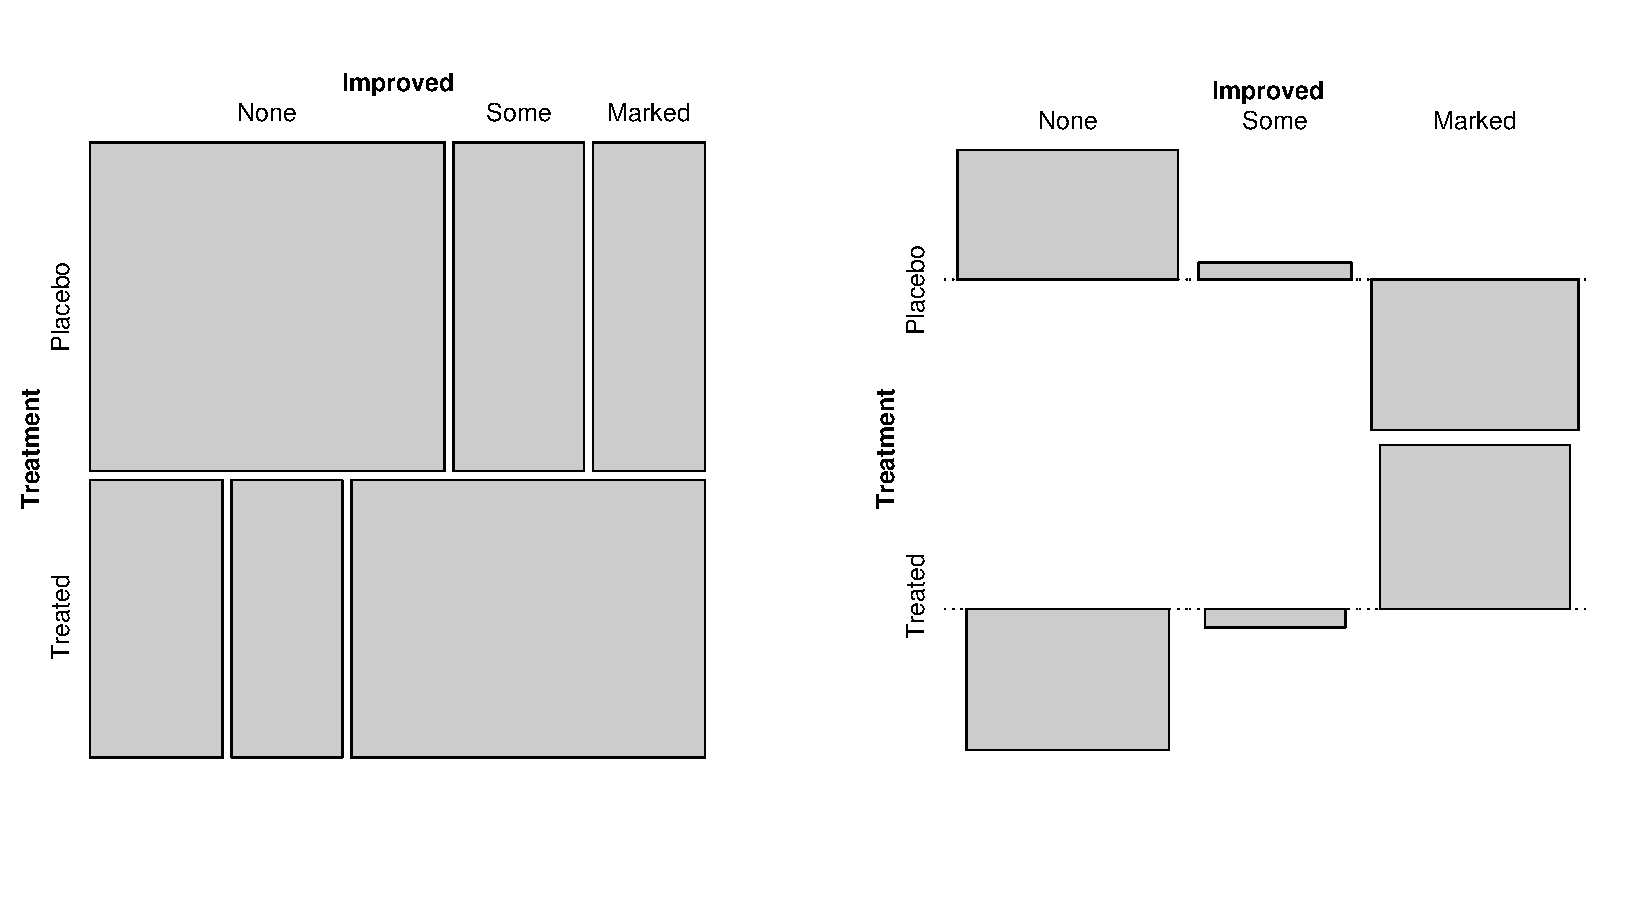
\includegraphics{residual-shadings-Arthritis-classic1}
\caption{Classic mosaic and association plot for the arthritis data.}
\label{fig:classic}
\end{center}
\end{figure}

For 2-way tables, \cite{vcd:Zeileis+Meyer+Hornik:2005} suggest to extend the
shading of \cite{vcd:Friendly:1994} to also visualize the outcome of an independence
test---either using the sum of squares of the Pearson residuals as the test statistic
or their absolute maximum. Both statistics and their corresponding (approximate) permutation
distribution can easily be computed using the function \code{coindep_test()}. Its arguments
are a contingency table, a specification of margins used for conditioning (only for conditional
independence models), a functional for aggregating the Pearson residuals (or alternatively the
raw counts) and the number of permutations that should be drawn. The conditional table needs
to be a 2-way table and the default is to compute the maximum statistic (absolute maximum of
Pearson residuals). For the Arthritis data, both, the maximum test

\begin{Schunk}
\begin{Sinput}
> set.seed(rseed)
> (art_max <- coindep_test(art, n = 5000))
\end{Sinput}
\begin{Soutput}
	Permutation test for conditional independence

data:  art 
f(x) = 1.8696, p-value = 0.0096
\end{Soutput}
\end{Schunk}

and the sum-of-squares test, indicate a significant departure from independence. 

\begin{Schunk}
\begin{Sinput}
> ss <- function(x) sum(x^2)
> set.seed(rseed)
> coindep_test(art, n = 5000, indepfun = ss)
\end{Sinput}
\begin{Soutput}
	Permutation test for conditional independence

data:  art 
f(x) = 11.2962, p-value = 0.0032
\end{Soutput}
\end{Schunk}

Thus, it can be concluded that the treatment is effective and leads to significantly more
improvement than the placebo. The classic views from Figure~\ref{fig:classic} and the inference
above can also be combined, e.g., using the maximum shading that highlights the cells in
an association or mosaic plot when the associated residuals exceed critical values of the
maximum test (by default at levels 90\% and 99\%). To compare this shading (using either HSV
or HCL colors) with the Friendly shading (using HSV colors), we generate all three versions
of the mosaic plot:

\begin{Schunk}
\begin{Sinput}
> mosaic(art, gp = shading_Friendly(lty = 1, eps = NULL))
> mosaic(art, gp = shading_hsv, gp_args = list(interpolate = art_max$qdist(c(0.9, 
+     0.99)), p.value = art_max$p.value))
> set.seed(rseed)
> mosaic(art, gp = shading_max, gp_args = list(n = 5000))
\end{Sinput}
\end{Schunk}

the  results are shown in the upper row of Figure~\ref{fig:shadings}. The last plot could
hae also been generated analogously to the second plot using \code{shading_hcl()} instead of
\code{shading_hsv()}---\code{shading_max()} is simply a wrapper function which performs the
inference and then visualizes it based on HCL colors.


\section{Piston rings data} \label{sec:arthritis}

Instead of bringing out the result of the maximum test in the shading, we could also use
a sum-of-squares shading that visualizes the result of the sum-of-squares test. As an illustration,
we use the \code{pistonrings} data from the \code{HSAUR} \citep{vcd:Everitt+Hothorn:2006}
package giving the number of piston ring failurs in different legs of different compressors
at an industry plant:

\begin{Schunk}
\begin{Sinput}
> data("pistonrings", package = "HSAUR")
> pistonrings
\end{Sinput}
\begin{Soutput}
          leg
compressor North Centre South
        C1    17     17    12
        C2    11      9    13
        C3    11      8    19
        C4    14      7    28
\end{Soutput}
\end{Schunk}

\begin{sidewaysfigure}[p]
\begin{center}
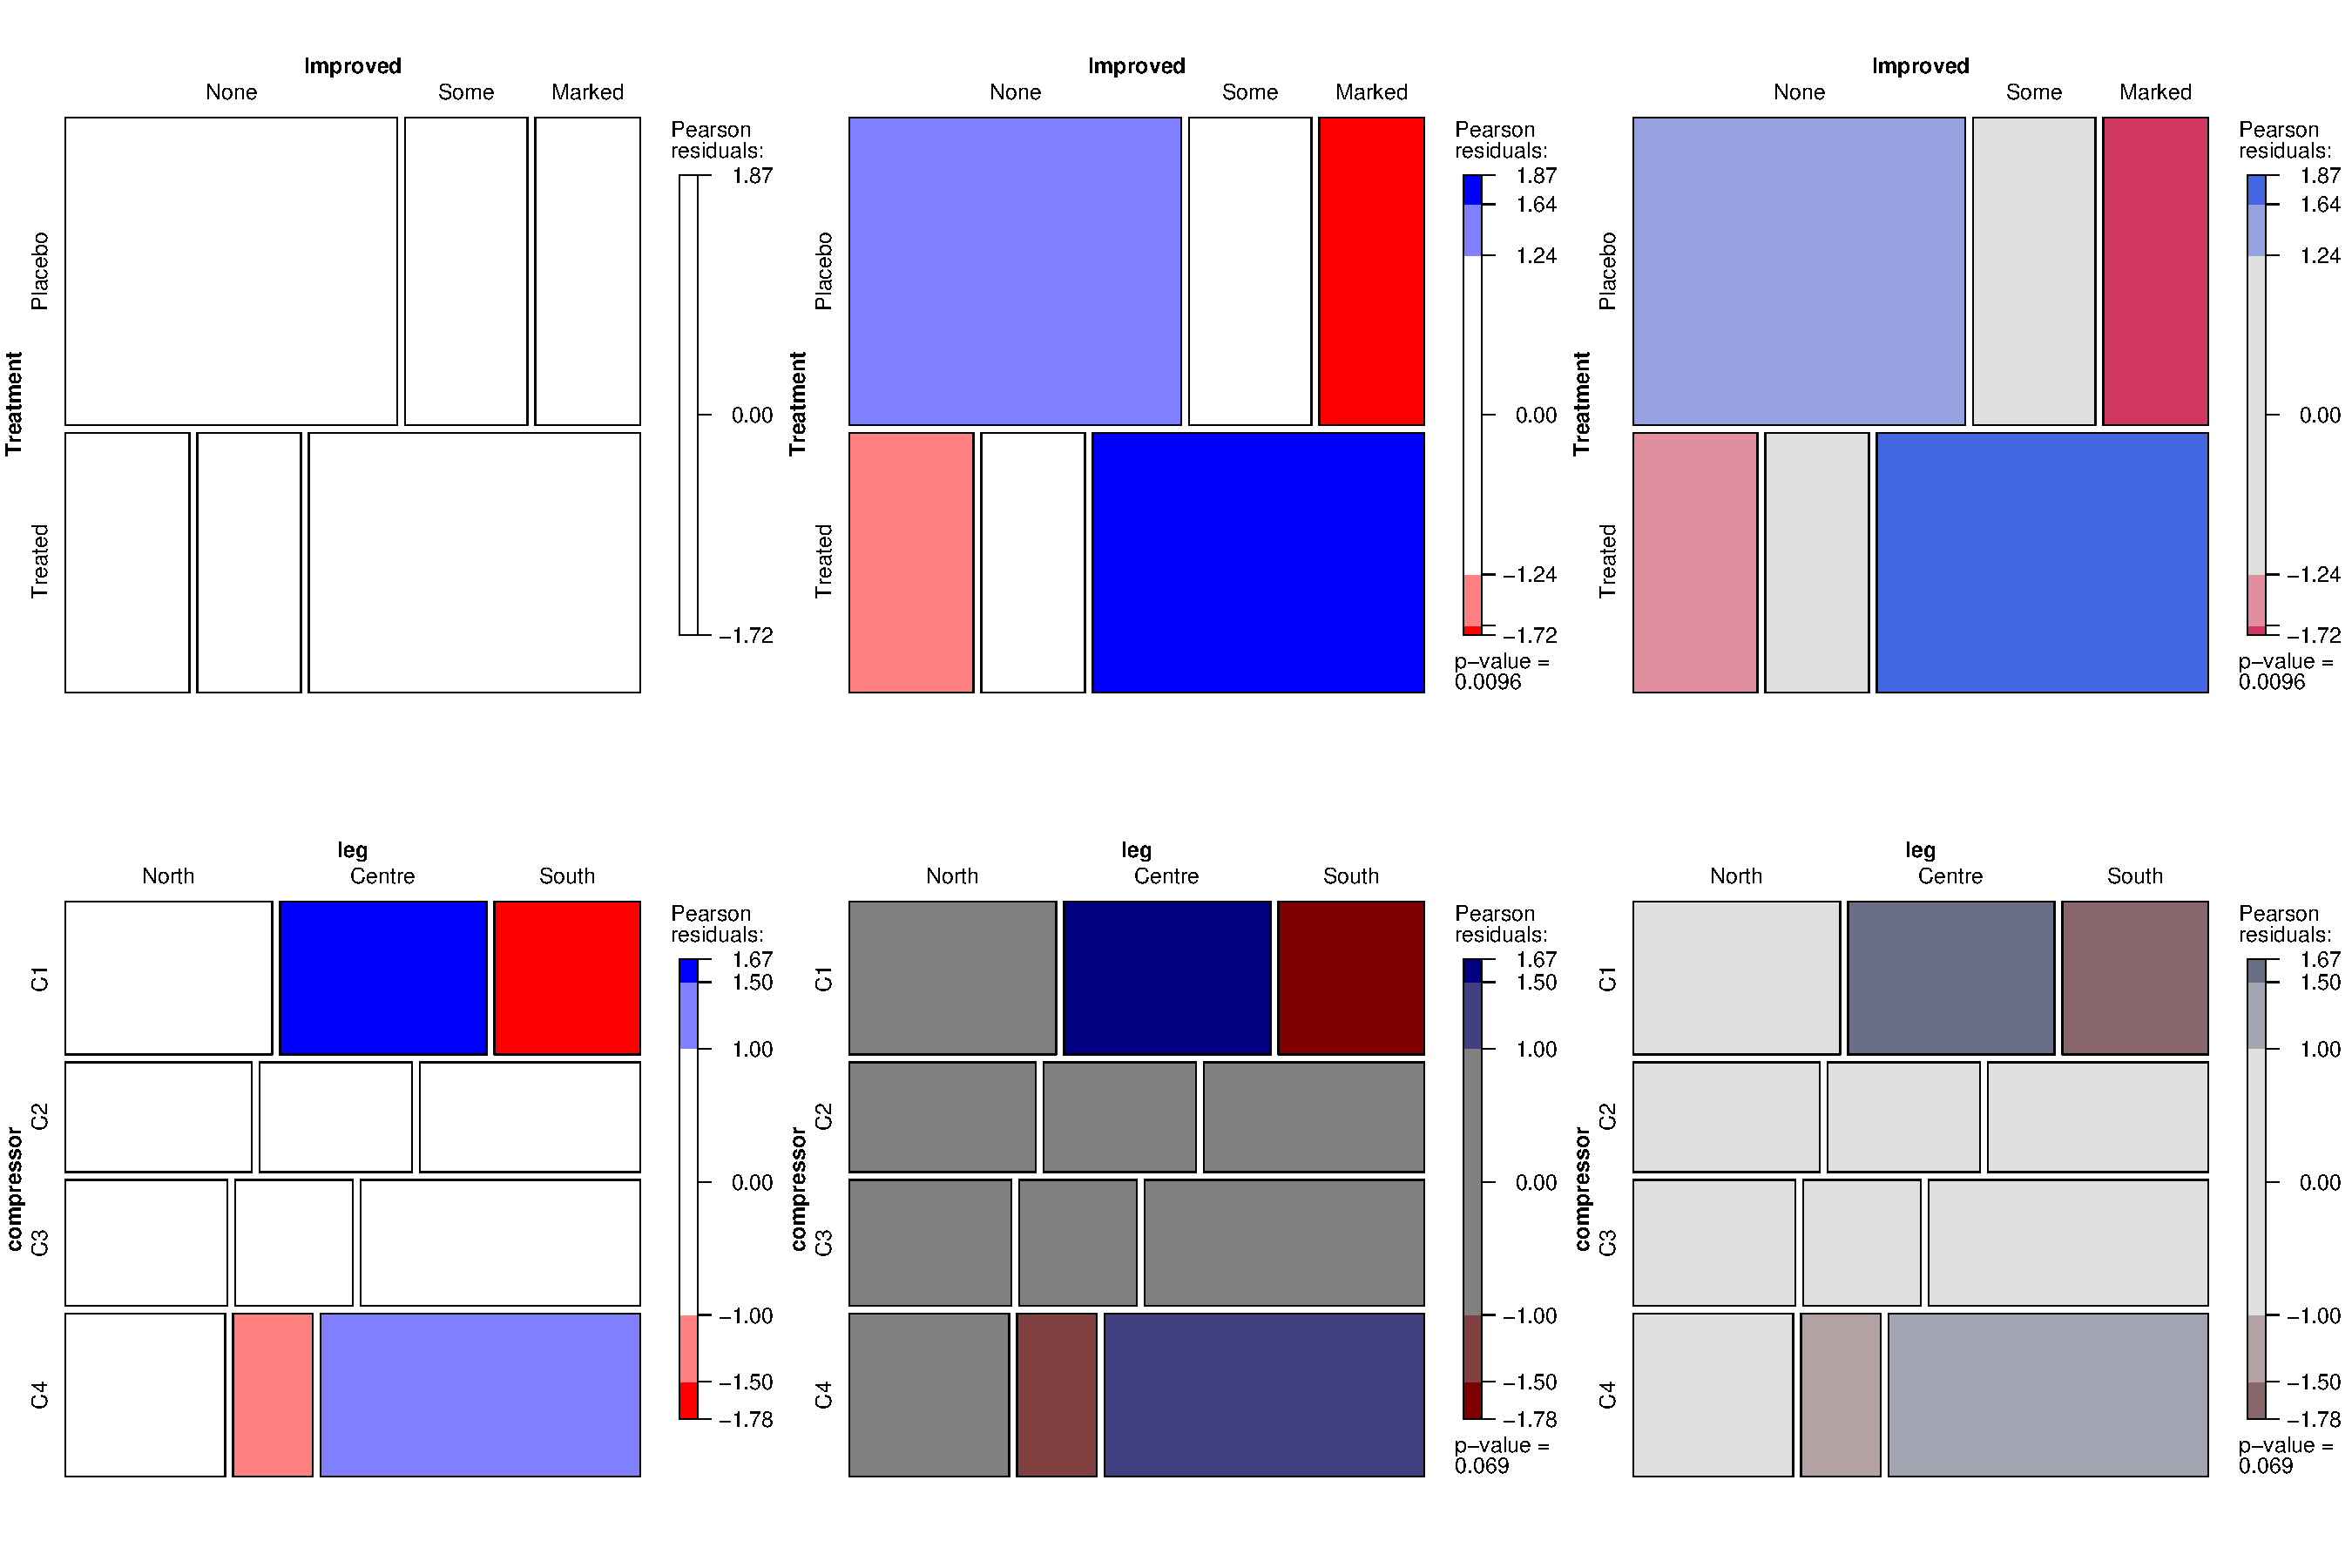
\includegraphics[width=.9\textwidth,keepaspectratio]{residual-shadings-shadings}
\caption{Upper row: Mosaic plot for the arthritis data with Friendly shading (left),
HSV maximum shading (middle), HCL maximum shading (right). Lower row: Mosaic
plot for the piston rings data with fixed user-defined cut offs 1 and 1.5 and 
Friendly shading (left), HSV sum-of-squares shading (middle), HCL sum-of-squares shading
(right).}
\label{fig:shadings}
\end{center}
\end{sidewaysfigure}

Although there seems to be some slight association between the leg (especially center and South)
and the compressor (especially numbers 1 and 4), there is no significant deviation from
independence:

\begin{Schunk}
\begin{Sinput}
> set.seed(rseed)
> coindep_test(pistonrings, n = 5000)
\end{Sinput}
\begin{Soutput}
	Permutation test for conditional independence

data:  pistonrings 
f(x) = 1.7802, p-value = 0.112
\end{Soutput}
\begin{Sinput}
> set.seed(rseed)
> (pring_ss <- coindep_test(pistonrings, n = 5000, indepfun = ss))
\end{Sinput}
\begin{Soutput}
	Permutation test for conditional independence

data:  pistonrings 
f(x) = 11.7223, p-value = 0.069
\end{Soutput}
\end{Schunk}

This can also be brought out graphically in a shaded mosaicplot by enhancing the Friendly
shading (based on the user-defined cut-offs 1 and 1.5, here) to use a less colorful palette,
either based on HSV or HCL colors:

\begin{Schunk}
\begin{Sinput}
> mosaic(pistonrings, gp = shading_Friendly(lty = 1, eps = NULL, 
+     interpolate = c(1, 1.5)))
> mosaic(pistonrings, gp = shading_hsv, gp_args = list(p.value = pring_ss$p.value, 
+     interpolate = c(1, 1.5)))
> mosaic(pistonrings, gp = shading_hcl, gp_args = list(p.value = pring_ss$p.value, 
+     interpolate = c(1, 1.5)))
\end{Sinput}
\end{Schunk}

The resulting plots can be found in the lower row of Figure~\ref{fig:shadings}. The default
in \code{shading_hcl()} and \code{shading_hsv()} is to use the asymptotical $p$~value, hence
we set it explicitely to the permtuation-based $p$~value computed above.



\section{Alzheimer and smoking} \label{sec:alzheimer}

For illustrating that the same ideas can be employed for visualizing (conditional)
independence in multi-way tables, \cite{vcd:Zeileis+Meyer+Hornik:2005} use a
3-way and a 4-way table. The former is taken from a case-control study of smoking
and {A}lzheimer's disease (stratified by gender). The data set is available in \proglang{R}
in the package \pkg{coin} \cite{vcd:Hothorn+Hornik+VanDeWiel:2006}.

\begin{Schunk}
\begin{Sinput}
> data("alzheimer", package = "coin")
> alz <- xtabs(~smoking + disease + gender, data = alzheimer)
> alz
\end{Sinput}
\begin{Soutput}
, , gender = Female

       disease
smoking Alzheimer's Other dementias Other diagnoses
  None           91              55              80
  <10             7               7               3
  10-20          15              16              25
  >20            21               9               9

, , gender = Male

       disease
smoking Alzheimer's Other dementias Other diagnoses
  None           35              24              24
  <10             8               1               2
  10-20          15              17              22
  >20             6              35              11
\end{Soutput}
\end{Schunk}

\begin{figure}[b!]
\begin{center}
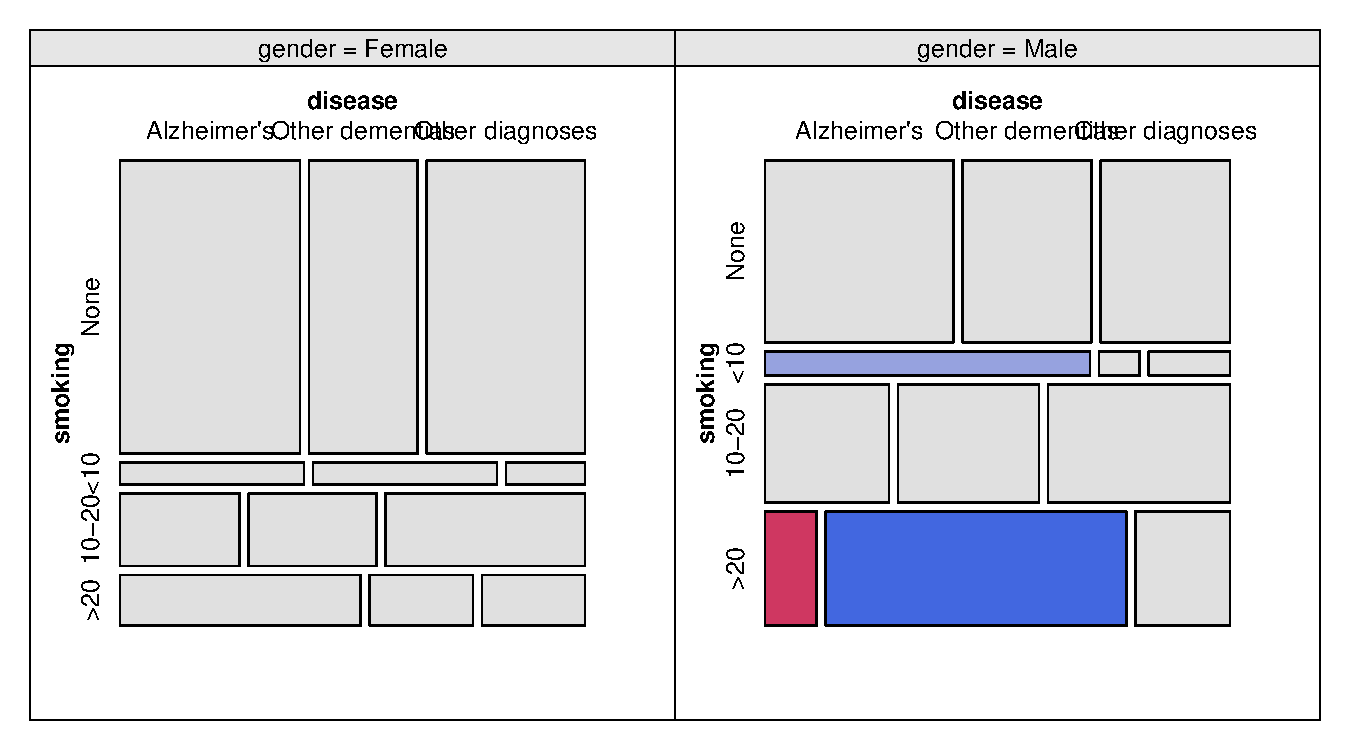
\includegraphics{residual-shadings-alzheimer-plot1}
\caption{Conditional mosaic plot with double maximum shading for conditional
independence of smoking and disease given gender.}
\label{fig:alz}
\end{center}
\end{figure}

To assess whether smoking behaviour and disease status are conditionally independent
given gender, \cite{vcd:Zeileis+Meyer+Hornik:2005} use three different types of test
statistics: double maximum (maximum of maximum statistics in the two strata), 
maximum sum of squares (maximum of sum-of-squares statistics), and sum of squares
(sum of sum-of-squares statistics). All three can be computed and assessed via
permutation methods using the function \code{coindep_test()}:

\begin{Schunk}
\begin{Sinput}
> set.seed(rseed)
> coindep_test(alz, 3, n = 5000)
\end{Sinput}
\begin{Soutput}
	Permutation test for conditional independence

data:  alz 
f(x) = 3.348, p-value < 2.2e-16
\end{Soutput}
\begin{Sinput}
> set.seed(rseed)
> coindep_test(alz, 3, n = 5000, indepfun = ss)
\end{Sinput}
\begin{Soutput}
	Permutation test for conditional independence

data:  alz 
f(x) = 35.8674, p-value < 2.2e-16
\end{Soutput}
\begin{Sinput}
> set.seed(rseed)
> coindep_test(alz, 3, n = 5000, indepfun = ss, aggfun = sum)
\end{Sinput}
\begin{Soutput}
	Permutation test for conditional independence

data:  alz 
f(x) = 46.8285, p-value < 2.2e-16
\end{Soutput}
\end{Schunk}

The conditional mosaic plot in Figure~\ref{fig:alz}
shows clearly that the association of smoking and disease is present only in
the group of male patients. The double maximum shading employed allows for
identification of the male heavy smokers as the cells `responsible' for the dependence:
other dementias are more frequent and Alzheimer's disease less frequent in this group than expected
under independence. Interestingly, there seems to be another large residual for
the light smoker group ($<$10 cigarettes) and Alzheimer's disease---however, this
is only significant at 10\% and not at the 1\% level as the other two cells.

\begin{Schunk}
\begin{Sinput}
> set.seed(rseed)
> cotabplot(~smoking + disease | gender, data = alz, panel = cotab_coindep, 
+     n = 5000)
\end{Sinput}
\end{Schunk}


\section{Corporal punishment of children}

As a 4-way example, data from a study of the Gallup Institute in Denmark in 1979 about
the attitude of a random sample of 1,456 persons towards corporal
punishment of children is used. The contingency table comprises four margins:
memory of punishments as a child (yes/no), attitude as a binary variable
(approval of ``moderate'' punishment or ``no'' approval), highest level
of education (elementary/secondary/high), and age group (15--24, 25--39, $\ge$40 years).

\begin{Schunk}
\begin{Sinput}
> data("Punishment", package = "vcd")
> pun <- xtabs(Freq ~ memory + attitude + age + education, data = Punishment)
> ftable(pun, row.vars = c("age", "education", "memory"))
\end{Sinput}
\begin{Soutput}
                        attitude  no moderate
age   education  memory                      
15-24 elementary yes               1       21
                 no               26       93
      secondary  yes               2        5
                 no               23       45
      high       yes               2        1
                 no               26       19
25-39 elementary yes               3       41
                 no               46      119
      secondary  yes               8       20
                 no               52       84
      high       yes               6        4
                 no               24       26
40-   elementary yes              20      143
                 no              109      324
      secondary  yes               4       20
                 no               44       56
      high       yes               1        8
                 no               13       17
\end{Soutput}
\end{Schunk}

It is of interest whether there is an association between memories of corporal punishments
as a child and attitude towards punishment of children as an adult, controlling
for age and education. All three test statistics already used above confirm that 
memories and attitude are conditionally associated:

\setkeys{Gin}{width=\textwidth}
\begin{figure}[t!]
\begin{center}
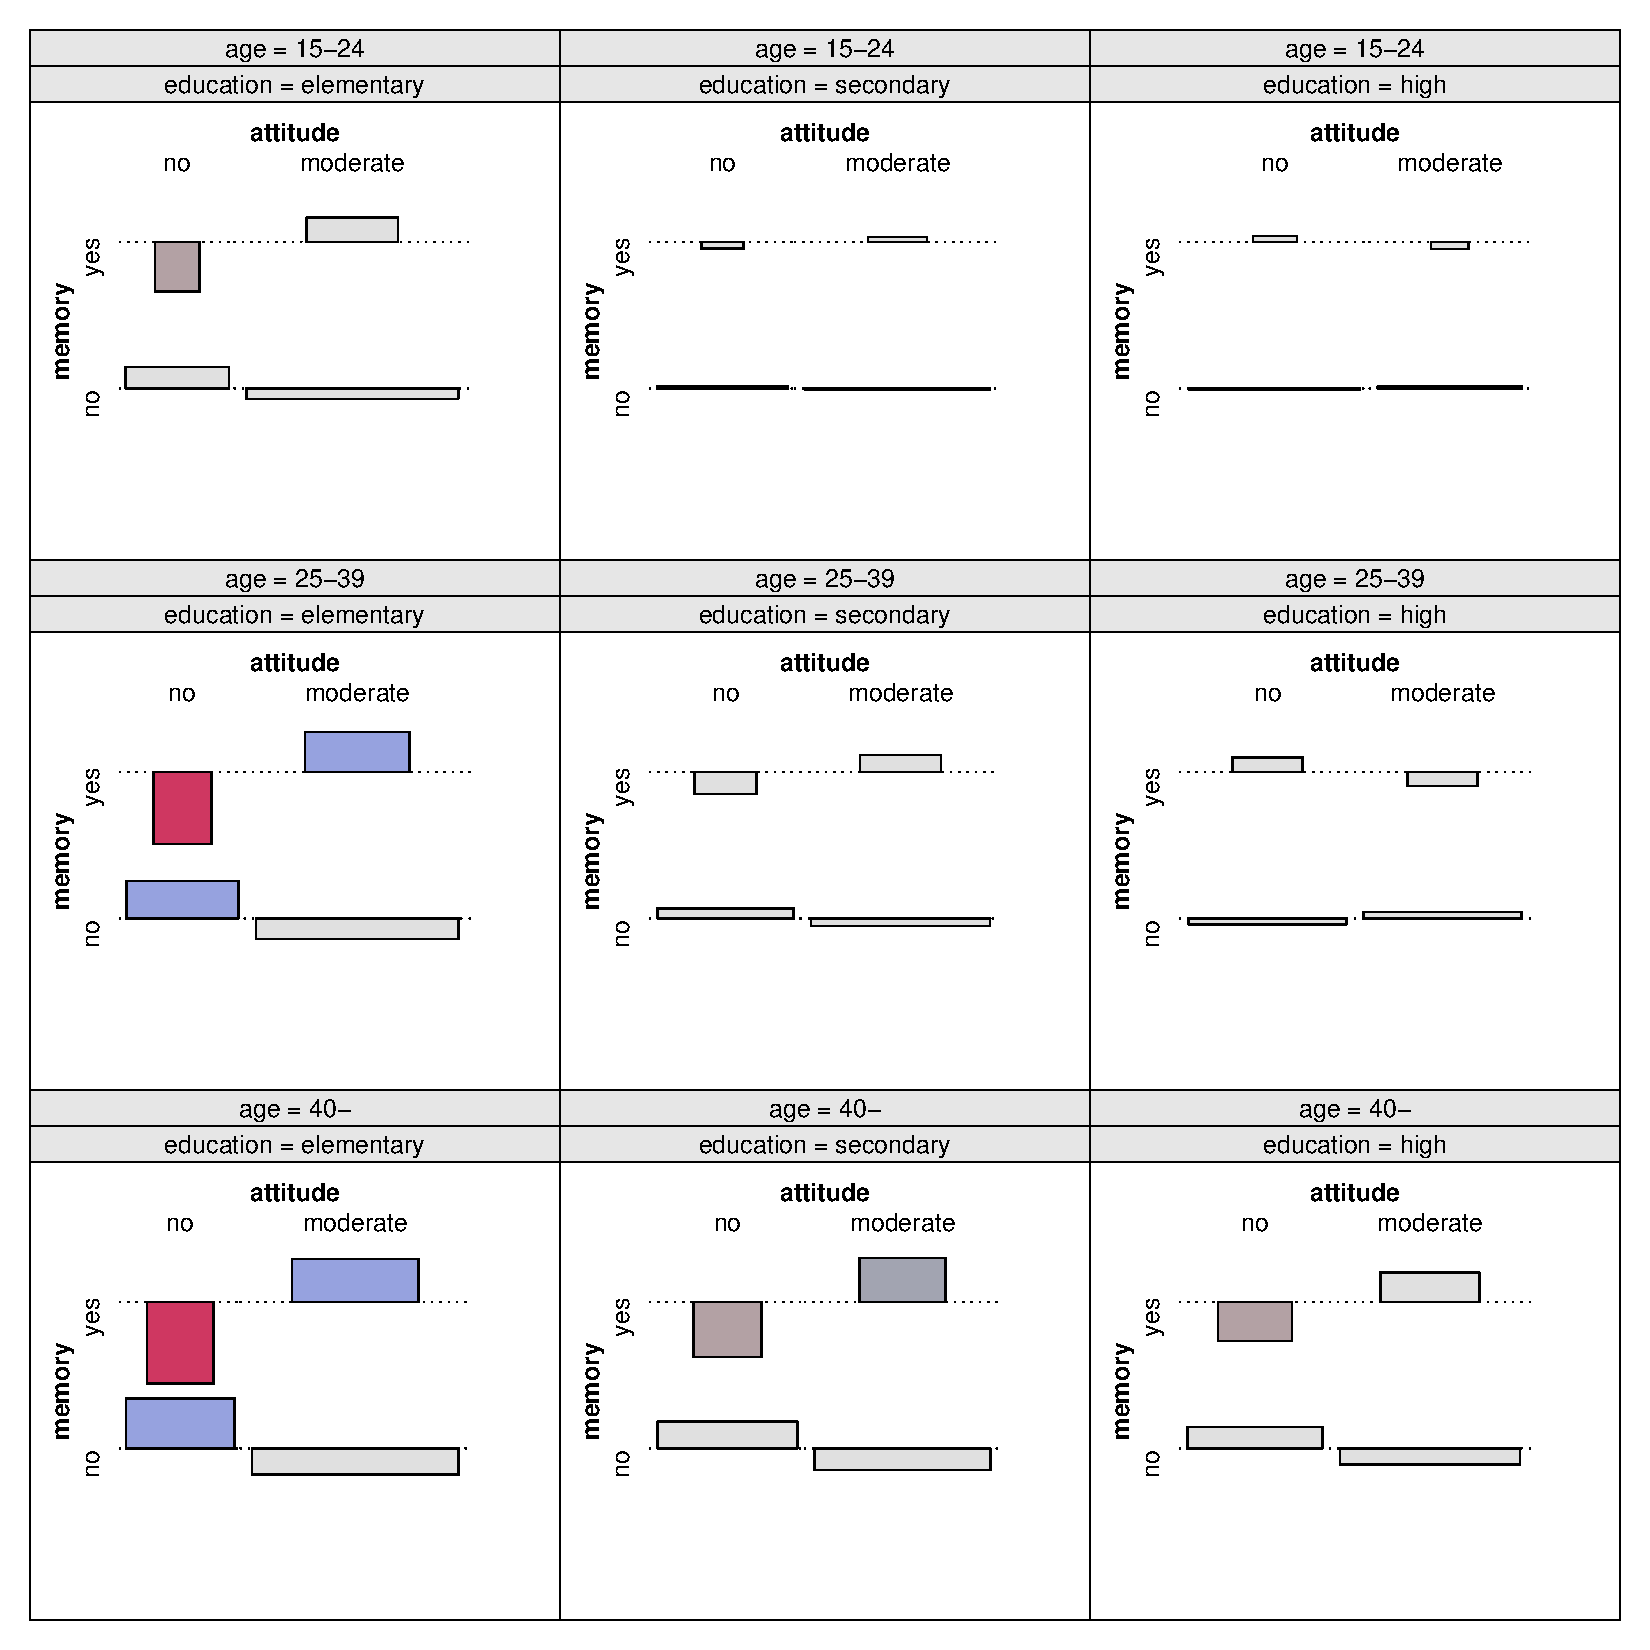
\includegraphics{residual-shadings-Punishment-assoc1}
\caption{Conditional association plot with maximum sum-of-squares shading for conditional
independence of memory and attitude given age and education.}
\label{fig:pun}
\end{center}
\end{figure}

\setkeys{Gin}{width=\textwidth}
\begin{figure}[t!]
\begin{center}
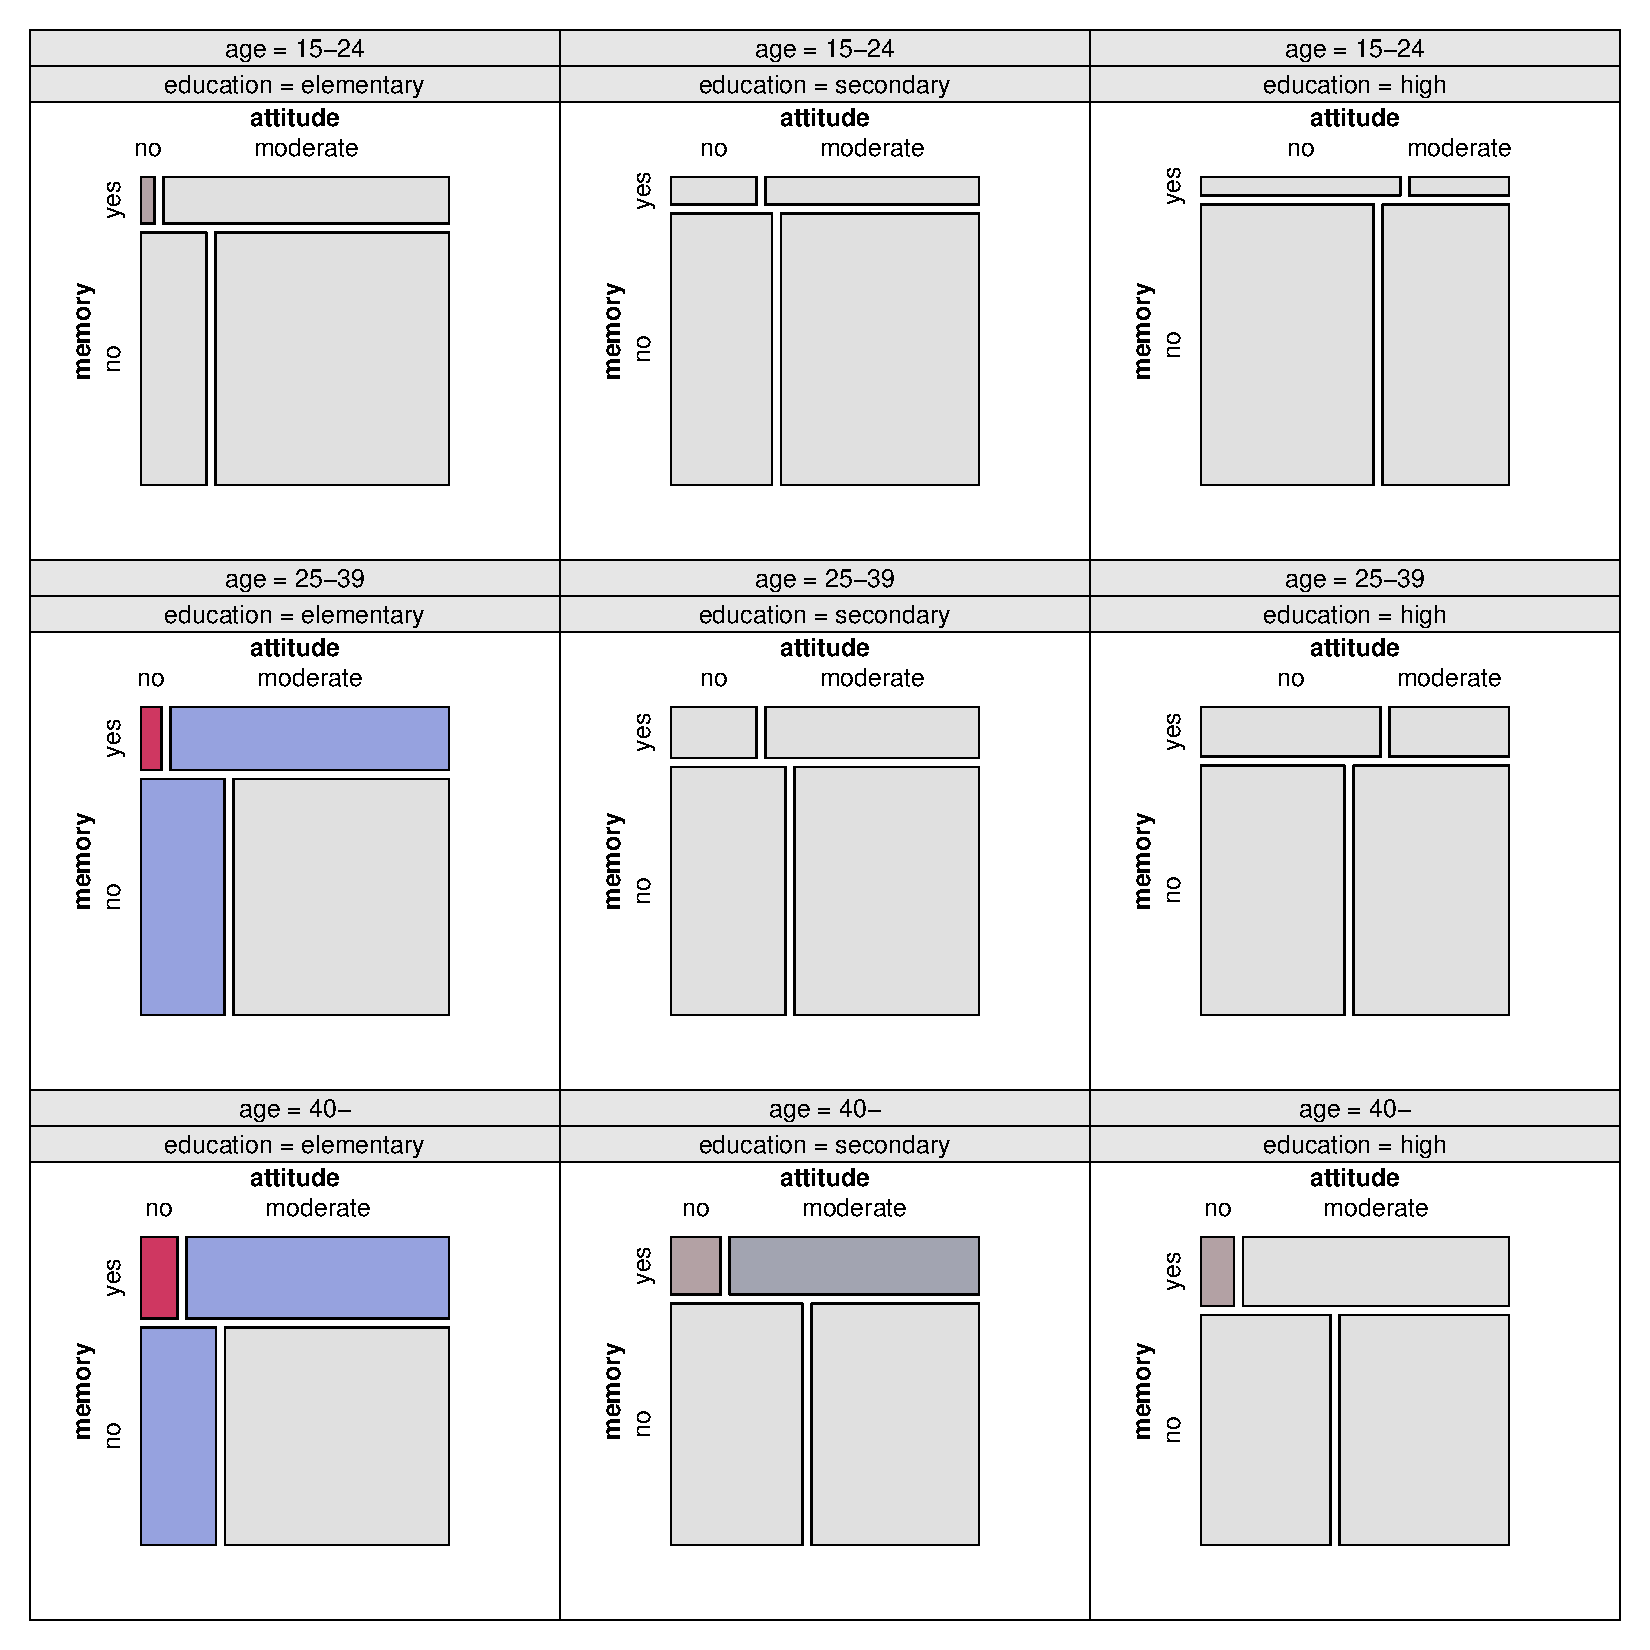
\includegraphics{residual-shadings-Punishment-mosaic1}
\caption{Conditional mosaic plot with maximum sum-of-squares shading for conditional
independence of memory and attitude given age and education.}
\label{fig:pun2}
\end{center}
\end{figure}

\begin{Schunk}
\begin{Sinput}
> set.seed(rseed)
> coindep_test(pun, 3:4, n = 5000)
\end{Sinput}
\begin{Soutput}
	Permutation test for conditional independence

data:  pun 
f(x) = 2.5725, p-value = 0.0056
\end{Soutput}
\begin{Sinput}
> set.seed(rseed)
> coindep_test(pun, 3:4, n = 5000, indepfun = ss)
\end{Sinput}
\begin{Soutput}
	Permutation test for conditional independence

data:  pun 
f(x) = 11.6256, p-value = 0.0064
\end{Soutput}
\begin{Sinput}
> set.seed(rseed)
> coindep_test(pun, 3:4, n = 5000, indepfun = ss, aggfun = sum)
\end{Sinput}
\begin{Soutput}
	Permutation test for conditional independence

data:  pun 
f(x) = 34.6041, p-value = 2e-04
\end{Soutput}
\end{Schunk}

Graphically, this dependence can be brought out using conditional association
or mosaic plots as shown in Figure~\ref{fig:pun} and \ref{fig:pun2}, respectively.
Both reveal an association between memories and attitude
for the lowest education group (first column) and highest age group (last row):
experienced violence seems to engender violence again as there are less adults
that disapprove punishment in the group with memories of punishments than expected
under independence. For the remaining four age-education groups, there seems to be
no association: all residuals of the conditional independence model are very close to
zero in these cells. The figures employ the maximum sum-of-squares shading
with user-defined cut offs 1 and 2, chosen to be within the range of the residuals.
The full-color palette is used only for those strata associated with a
sum-of-squares statistic significant at (overall) 5\% level, the reduced-color
palette is used otherwise. This highlights that the dependence pattern is significant
only for the middle and high age group in the low education column. The other panels
in the first column and last row also show a similar dependence pattern, however, it is not
significant at 5\% level and hence graphically down-weighted by using reduced color.

\begin{Schunk}
\begin{Sinput}
> set.seed(rseed)
> cotabplot(~memory + attitude | age + education, data = pun, panel = cotab_coindep, 
+     n = 5000, type = "assoc", test = "maxchisq", interpolate = 1:2)
\end{Sinput}
\end{Schunk}
\begin{Schunk}
\begin{Sinput}
> set.seed(rseed)
> cotabplot(~memory + attitude | age + education, data = pun, panel = cotab_coindep, 
+     n = 5000, type = "mosaic", test = "maxchisq", interpolate = 1:2)
\end{Sinput}
\end{Schunk}


\bibliography{vcd}

\end{document}
